% Vector workflow for the Voltera report. No customer data or model results.
\documentclass[tikz,border=4pt]{standalone}
\usepackage[T1]{fontenc}
\usepackage{lmodern}
\usetikzlibrary{arrows.meta,positioning,calc}
\begin{document}
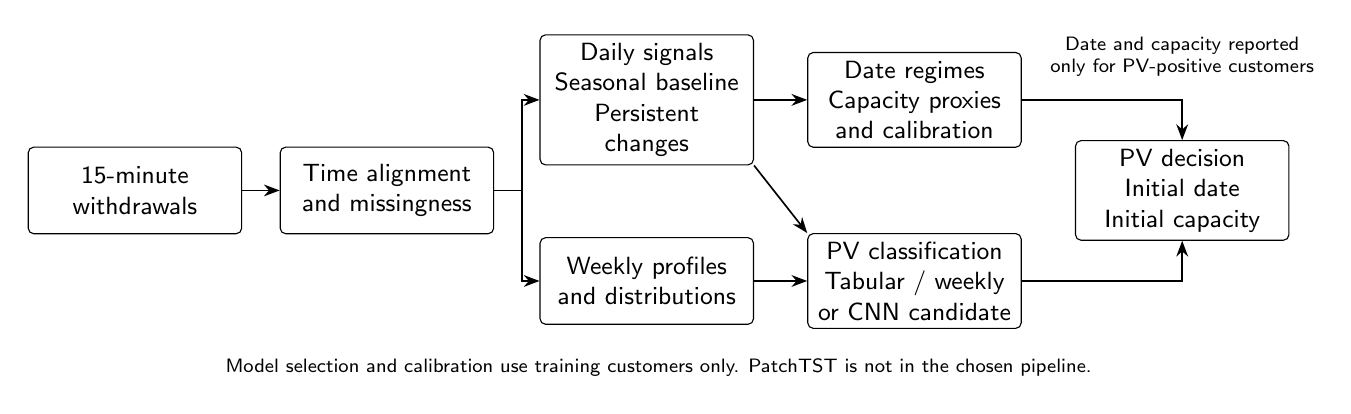
\begin{tikzpicture}[
  font=\sffamily\small,
  stage/.style={draw,rounded corners=2pt,align=center,text width=25mm,minimum height=11mm,inner sep=3pt},
  flow/.style={-{Stealth[length=2mm]},semithick},
  note/.style={font=\sffamily\scriptsize,align=center}
]
\node[stage] (input) at (0,0) {15-minute\\withdrawals};
\node[stage] (prep) at (3.2,0) {Time alignment\\and missingness};
\node[stage] (physical) at (6.5,1.15) {Daily signals\\Seasonal baseline\\Persistent changes};
\node[stage] (weekly) at (6.5,-1.15) {Weekly profiles\\and distributions};
\node[stage] (estimates) at (9.9,1.15) {Date regimes\\Capacity proxies\\and calibration};
\node[stage] (presence) at (9.9,-1.15) {PV classification\\Tabular / weekly\\or CNN candidate};
\node[stage] (output) at (13.3,0) {PV decision\\Initial date\\Initial capacity};
\draw[flow] (input) -- (prep);
\draw[flow] (prep.east) -- ++(0.35,0) |- (physical.west);
\draw[flow] (prep.east) -- ++(0.35,0) |- (weekly.west);
\draw[flow] (physical) -- (estimates);
\draw[flow] (weekly) -- (presence);
\draw[flow] (physical.south east) -- (presence.north west);
\draw[flow] (estimates.east) -- ++(0.3,0) -| (output.north);
\draw[flow] (presence.east) -- ++(0.3,0) -| (output.south);
\node[note] at (13.3,1.7) {Date and capacity reported\\only for PV-positive customers};
\node[note] at (6.65,-2.25) {Model selection and calibration use training customers only. PatchTST is not in the chosen pipeline.};
\end{tikzpicture}
\end{document}
